% A workaround to allow relative paths in included subfiles
% that are to be compiled separately
% See https://tex.stackexchange.com/questions/153312/subfiles-inside-a-subfile-using-relative-paths
\providecommand{\main}{..}
\documentclass[\main/thesis.tex]{subfiles}

\begin{document}

\chapter{Matrix Multiplication}
\label{cha:matmul}

Matrix multiplication, as a critical operation in many applications, has been the focus of optimisation research for decades.
\bk{Can I just leave it at that or do I need to provide some random citations proving my point?}
Simple insights into matrix multiplication have enabled better data usage, both spatially and temporally, via optimisations such as loop switching and loop unrolling.
Contemporary libraries and their overall frameworks are derived from seminal work by Goto and van de Geijn~\autocite{goto2008anatomy}.
More recent work~\autocite{vanzee2015blis,zee2016blis}\todo{More citations, not just BLIS works.} have improved upon that seminal work, but the overall structure remains the same.
\ik{The main direction of contributions is to make these frameworks easier to port to target architectures by providing a modular approach for the microkernel. Low et al.~\autocite{low2016analytical} showed that the parameters of the microkernels in BLIS can be determined analytically.}

Goto and van de Geijn's work concludes that matrix multiplication should be implemented in a \emph{layered approach}.
Each of these ``layers'' is typically one or more loops that perform some function before executing the enclosed layer.
It can be convenient to think of each of the upper layers as a function with a nested function call within it.
The innermost layer in this view performs the most basic computation on which the entire operation is built, essentially a small and fast matrix multiplication.
The surrounding layers are concerned with the optimisation of data movement and layout.

Typically, the layered approach consists of two layers:
\begin{enumerate*}[itemjoin={{; }}, itemjoin*={{; and }}, label=\textbf{(\arabic*)}, after={.}]
  \item the blocking strategy responsible for breaking up the computation combined with the packing strategy responsible for optimising data movement between memory and cache as well as data layout within the cache (the \emph{outer kernel} or \emph{macro kernel})
  \item the computation strategy responsible for data movement between cache and register as well as for producing the actual result (the \emph{inner kernel} or \emph{micro kernel})
\end{enumerate*}
This work focuses on building a modular innermost layer and therefore the outer layer is explained only briefly for completeness.

\section{The Outer Kernel}
The outer kernel is a delicate dance between blocking and packing.
Blocking takes an operation and breaks it into smaller pieces, focusing on computing output in a piecewise manner rather than all at once.
Packing takes the operands of an operation and duplicates data into a smaller buffer where elements are more likely to fit in cache simultaneously, allowing faster access times.
\bk{
  Is this enough explanation of what blocking and packing are?
  It seems orthogonal to the rest of the thesis so I'd like to avoid going too in depth if possible.
}
If the blocking factor is too large (\ie many, small blocks) then there is an excessive amount of data movement, requiring packing more often with less reuse of each packed element.
However, when the blocking is too small (\ie few, large blocks) then blocks no longer fit in cache -- in the worst case, causing page faults -- and packing is ineffective.

\ik{The outer kernel consists of three nested loops (one for each computation dimension) and packing function calls.
As the matrix sizes typically found in application are much bigger than what data cache can fit, the three loops serve to divide the task into smaller portions (blocks).
The sizes of the blocks are determined by the sizes of L1, L2 and L3 caches so to maximize cache utilization.
However, accesses to these smaller portions would put stress on the TLB as data in the blocks lies with the original stride, which is large.
Packing (copying matrix to a buffer with specific storage layout) was introduced to use the minimum number of memory pages and to place matrix elements in the order they will be later accessed by the inner kernel to improve data locality.
The work of Goto and Van de Geijn~\autocite{goto2008anatomy} outlines several possibilities to pack the input matrices but identifies one that is most promising.
For that case, matrices A and B are copied to two other memory buffers (blocks) so that elements in these blocks lie contiguously.
}

Goto and van de Geijn address blocking, caching and \gls{tlb} issues in their work by devising three ways of breaking up both operands and output.
\bk{Can TLB remain a glossary entry or is further explanation required here.}
\ik{TLB should remain a glossary entry as Goto's paper introduces TLB and its relation to the whole process}
When blocking, each new blocking loop breaks up a single dimension of the multiplication.
Dividing one dimension of a matrix produces a \emph{panel}: a section with one long dimension and one short dimension.
Further dividing a panel produces a section with two short dimensions called a block.
Only two of the three dimensions ($M$, $K$, $N$) are blocked while the third is the inner most loop's iteration variable.
This produces ${3 \choose 2}=3$ different innermost loops\footnotemark.
\footnotetext{``Three choose two''.}
Different combinations of blocking orders also induce different packing choices that change which of $A$, $B$, and $C$ are packed into L1 and L2 cache.

\subsection{Blocking and Packing for Cache}
\label{sec:blockPack}
\bk{
  I kind of don't like the rest of this section.
  It just seems like a summary of the Goto paper while also lacking the completeness of their work.
  I think it's important for the summary of \code{GEPDOT}, but I'm unsure if the rest of it is truly important.
  Maybe it's fine because it's not the focus of the paper, as stated above.
}
The primary concern when blocking and packing for cache is optimising L2 cache bandwidth.
When dimensions $M$ and $N$ are blocked, the innermost loop multiplies a panel by another panel, producing a block.
This breakdown is called \code{GEPDOT} because it computes the dot product of two panels.
According to their proposed method, with this breakdown, $C$ will be packed in L2 cache.
Unfortunately, because \gls{gemm} is an accumulating operation (\eg $C \mathrel{+}= AB$), $C$ must be read from cache and then written back.
When either $A$ or $B$ are packed into L2 cache, as is the case in the other breakdowns, L2 cache is only read from.
In essence, this means that the \code{GEPDOT} method is less bandwidth efficient because it requires both a read and a write.
\bk{I need to rewrite the section in \rcha{mma} now that this is written.}

\ik{
  One of the key insights of the Goto and Van de Geijn's work~\autocite{goto2008anatomy} is that L2 utilization is the top priority for performance.
  The blocking and packing of matrices can come in different combinations of loops orders and matrix packing choices, as briefly mentioned above.
  Goto reasoned in~\autocite{goto2008anatomy} and devised that packing A, B in L2 and L3 caches is the best approach.
  Other combinations are symmetric to this approach except for one, commonly known as~\code{GEPDOT}.
  In that scenario, the matrix C is packed and loaded into L1 and L2 on each block iteration, while elements of A and B are streamed from memory.
  As compared to the implementation where either A or B resides in L2,~\code{GEPDOT} reads \textbf{and then writes} a few elements of C from L2 which results in twice the L2 bandwidth usage.
}
\ik{Just a note: even if it was matmul, not gemm, both GEPDOT and GEBP accumulate.}

Without loss of generality, an implementer can choose between the remaining two methods (blocking $M$ and $K$ or blocking $K$ and $N$) based on the storage order of $C$.
Within one of these methods, the order in which $K$ and the second dimension are blocked creates two options.
Given that one argument matrix is already packed in L2 cache, the first option, which blocks $M$ or $N$ then $K$,
\begin{enumerate*}[itemjoin*={{ and }}, label=\textbf{(\arabic*)}, after={.}]
  \item streams $C$ to and from memory
  \item packs the second argument matrix in L1 cache
\end{enumerate*}
Given again that one argument matrix is packed in L2 cache, the second option, which blocks $K$ followed by $M$ or $N$,
\begin{enumerate*}[itemjoin*={{ and }}, label=\textbf{(\arabic*)}, after={.}]
  \item streams the second argument matrix from memory
  \item computes $C$ in a temporary in L1 cache which is eventually unpacked and merged with $C$ in memory
\end{enumerate*}
The operations labeled \textbf{(1)} in each option can be assumed to have negligible impact because they can be pipelined with computation.
However, the operations labeled \textbf{(2)} are effectively overhead.
By virtue of the unpacking and merging of $C$ being a more complex operation, the first option for either blocking method is concluded to be superior.

\subsubsection{Blocking and Packing for Registers}
The dimensions chosen to maximise cache usage are likely to be too large for the registers to handle, thus a further set of loops can be added to block for registers.
These loops only block the pre-packed buffers in memory and do not perform any packing themselves.
Instead, when packing for the cache, the order in which data is packed is modified.
Rather than packing in the same order relative to the original data, data is organised such that these sub-matrix register arguments are contiguous.
Packing in this way results in only a single data copy and allows reads to register for calculation to be contiguous in memory.

\subsubsection{Practicality}
Na\"ive matrix multiplication (\ie \rlst{basicmatmul}) does not perform blocking nor packing; such a case can be viewed as a ``bare'' inner kernel, without an outer kernel.
Given small matrices as operands, this is often the correct choice.
The overhead resulting from the data movement in the outer kernel is designed to be overshadowed by the speed up gained from improved cache performance.
When input and output data begin small enough to be entirely resident in cache, the effort made to pack and block is shown to be an unnecessary expense.

However, given large matrices, lacking a blocking and packing layer is disastrous for performance.
With sufficiently large matrices, every load will result in a cache miss because the requested data will have been expelled from the cache by a more recent load simply by the pigeonhole principle.
In the worst case, these issues are compounded with \gls{tlb} misses as well.
Therefore, while a single, optimised inner kernel is always critical to performance, it is important for library implementers or compilers to consider the size of their data when possible and offer multiple outer-kernel data-management strategies.

\section{The Inner Kernel}
The inner kernel is focused on maximising performance.
Whether the computation itself has small dimensions or a larger computation has been blocked and packed by an outer kernel, the inner kernel is meant to be as tight and efficient as possible.
This means considering optimisations such as loop unrolling and instruction rescheduling to improve operation pipelining.
Hardware-wise, the instruction cache, instruction issue rate, register pressure, and functional unit availability must also be taken into account.

Unrolling the kernel to a larger degree allows for greater opportunities in instruction rescheduling.
Computations can be moved closer to loads to enable pipelining as well as interleaved to hide stalls due to occupied functional units.
Future iterations that would load the same data can also be moved such that the values are still in register and can be reused, reducing register pressure and stores.
However, unrolling too much can degrade instruction cache performance and bloat executable size.
\bk{I feel like there's more discussion to be had here, I just need to return with a clear mind.}

\subsection{Inner Product}
\bk{Content to be moved here.}

\subsection{Outer Product}
\bk{Content to be moved here.}

\subsection{Inner Product vs Outer Product}
\label{sec:products}
\begin{figure}[t]
 \hfill
  \begin{subfigure}{.45\linewidth}
    \centering
    \begin{tikzpicture}[scale=1/2]
      \draw[step=1, shift={(0, 3)}] (0, 0) grid +(4, 1);
      \node at (4.75, 2) {$\times$};
      \draw[step=1, shift={(5.5, 0)}] (0, 0) grid +(1, 4);
      \node at (7.25, 2) {$=$};
      \draw[step=1, shift={(8, 3)}] (0, 0) grid +(1, 1);
      \node at (2, 5) {$A$};
      \node at (6, 5) {$B$};
      \node at (8.5, 5) {$C$};
    \end{tikzpicture}
    \caption{Inner product.}
    \label{fig:innerProduct}
  \end{subfigure}
 \hfill
  \begin{subfigure}{.45\linewidth}
    \centering
    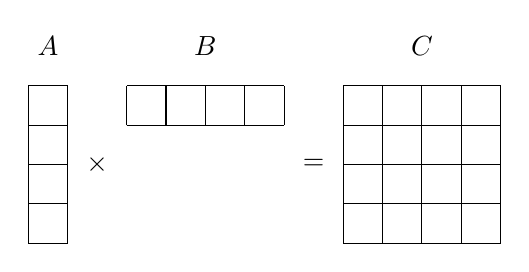
\begin{tikzpicture}[scale=1/2]
      \draw[step=1, shift={(0, 0)}] (0, 0) grid +(1, 4);
      \node at (1.75, 2) {$\times$};
      \draw[step=1, shift={(2.5, 3)}] (0, 0) grid +(4, 1);
      \node at (7.25, 2) {$=$};
      \draw[step=1, shift={(8, 0)}] (0, 0) grid +(4, 4);
      \node at (.5, 5) {$A$};
      \node at (4.5, 5) {$B$};
      \node at (10, 5) {$C$};
    \end{tikzpicture}
  \caption{Outer-product (rank-$1$ update) operation.}
    \label{fig:outerProduct}
  \end{subfigure}
  \hfill
  \caption{Example matrix-matrix multiplication computation styles.}
  \label{fig:product}
  \vspace{-0.15cm}
\end{figure}

Matrix multiplication's inner kernel is implementable through two operations: inner product and outer product.
Both operations arrive at the same destination albeit via different processes.
Consider \rfig{product}.
\rfig{innerProduct} illustrates the inner product: an element-wise multiplication between a row of matrix $A$ and a column of matrix $B$ followed by the summation of the products (\ie the dot product).
In short, two vectors produce a single, fully-computed output element.
This is the operation which usually first comes to mind when discussing matrix multiplication.
Computing the outer product, shown in \rfig{outerProduct}, results in a column of matrix $A$ and a row of matrix $B$ producing a \emph{partial} output matrix.
That is, a matrix whose elements are the result of a single product.
One such matrix is produced per combination of $A$ column and $B$ row; these matrices must be summed to produce the output $C$.

At the end of the computation, both methods will have performed exactly the same number of multiplications and additions.
As well, in a machine with unlimited resources, including vector registers of unlimited length, they will have performed the same number of stores and loads.
In such a theoretical framework, at least in terms of computations performed, neither method can be said to be better.
However, in a practical machine, it is impossible to load the entirety of a long row or of a long column into vector registers in order to fully compute a portion of the matrix.

Long dimension lengths make tiling a necessity.
Tiling, as discussed in \rsec{blockPack}, breaks the operation into smaller, more manageable operations.
As discussed in that same section, on the macro scale, Goto and van de Geijn conclude that a dot-product-based tiling results in more costly data movement, making it a poor choice.

When considering the micro scale, the dot-product approach also makes poor use of \gls{simd} capabilities.
Computing the dot product requires a horizontal reduction (or tree reduction): the reduction of all the \glspl{lane} of a vector register into a single scalar element.
Computing a partial result in this manner reduces the effectiveness of \gls{simd} by creating a scalar value.
\Gls{simd} was created specifically to alleviate the bottleneck associated with working with scalar values; reverting to scalars should therefore be avoided when possible.
The outer product, on the other hand, uses a vertical reduction (or element-wise reduction) that allows partial products to be accumulated simultaneously in all \glspl{lane} of the destination vector register.

\subsection{Goto and van de Geijn in the Inner Kernel}
\bk{This title could be shortened or tailored more.}
\begin{figure}[t]
  \hfill
  \begin{subfigure}{.45\linewidth}
    \centering
    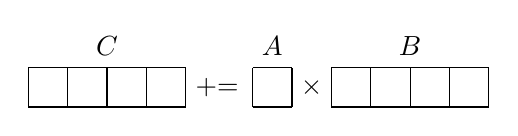
\begin{tikzpicture}[scale=1/2]
      \node[above=.75] at (2, 1) {$C$};
      \draw[shift={(0,0)}] (0,0) grid +(4,1);
      \node at (4.8,.5) {$\mathrel{+}=$};
      \node[above=.75] at (6.2, 1) {$A$};
      \draw[shift={(5.7,0)}] (0,0) grid +(1,1);
      \node at (7.2,.5) {$\times$};
      \node[above=.75] at (9.7, 1) {$B$};
      \draw[shift={(7.7,0)}] (0,0) grid +(4,1);
    \end{tikzpicture}
    \caption{Block times panel mathematically.}
    \label{fig:gebpMath}
  \end{subfigure}
  \hfill
  \begin{subfigure}{.45\linewidth}
    \centering
    \begin{tikzpicture}
      \draw[step=0.8cm,shift={(0,0)}] (0,0) grid +(.8cm,3.2cm);
      \matrix[matrix of nodes,matrix anchor=south west,inner sep=0pt,minimum height=.8cm,text width=.8cm,align=center,shift={(0,0)}]
      {
        $c_{0,0}$\\
        $c_{0,1}$\\
        $c_{0,2}$\\
        $c_{0,3}$\\
      };
      \node at (1.175cm, 1.6cm) {$\mathrel{+}=$};
      \draw[step=0.8cm,shift={(1.6cm,0)}] (0,0) grid +(.8cm,3.2cm);
      \matrix[matrix of nodes,matrix anchor=south west,inner sep=0pt,minimum height=.8cm,text width=.8cm,align=center,shift={(1.6cm,0)}]
      {
        $a_{0,0}$\\
        $a_{0,0}$\\
        $a_{0,0}$\\
        $a_{0,0}$\\
      };
      \node at (2.75, 1.6cm) {$\times$};
      \draw[step=0.8cm,shift={(3.1cm,0)}] (0,0) grid +(.8cm,3.2cm);
      \matrix[matrix of nodes,matrix anchor=south west,inner sep=0pt,minimum height=.8cm,text width=.8cm,align=center,shift={(3.1cm,0)}]
      {
        $b_{0,0}$\\
        $b_{0,1}$\\
        $b_{0,2}$\\
        $b_{0,3}$\\
      };
    \end{tikzpicture}
    \caption{Block times panel in register using \gls{simd} \acrshort{fma}.}
    \label{fig:gebpSimd}
  \end{subfigure}
  \hfill
  \caption[Block and panel kernel mathematically and in register]{Block times panel computation both mathematically and as computed by \glslink{broadcast}{broadcasting} and \acrshort{fma}.\bk{Better caption?}}
  \label{fig:gebp}
\end{figure}

\begin{figure}[t]
  \hfill
  \begin{subfigure}{.45\linewidth}
    \centering
    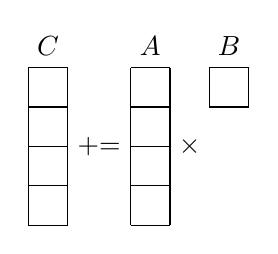
\begin{tikzpicture}[scale=1/2]
      \node[above=.75] at (.5, 4) {$C$};
      \draw[shift={(0,0)}] (0,0) grid +(1,4);
      \node at (1.8,2) {$\mathrel{+}=$};
      \node[above=.75] at (3.1, 4) {$A$};
      \draw[shift={(2.6,0)}] (0,0) grid +(1,4);
      \node at (4.1,2) {$\times$};
      \node[above=.75] at (5.1, 4) {$B$};
      \draw[shift={(4.6,3)}] (0,0) grid +(1,1);
    \end{tikzpicture}
    \caption{Panel times block mathematically.}
    \label{fig:gepbMath}
  \end{subfigure}
  \hfill
  \begin{subfigure}{.45\linewidth}
    \centering
    \begin{tikzpicture}
      \draw[step=0.8cm,shift={(0,0)}] (0,0) grid +(.8cm,3.2cm);
      \matrix[matrix of nodes,matrix anchor=south west,inner sep=0pt,minimum height=.8cm,text width=.8cm,align=center,shift={(0,0)}]
      {
        $c_{0,0}$\\
        $c_{1,0}$\\
        $c_{2,0}$\\
        $c_{3,0}$\\
      };
      \node at (1.175cm, 1.6cm) {$\mathrel{+}=$};
      \draw[step=0.8cm,shift={(1.6cm,0)}] (0,0) grid +(.8cm,3.2cm);
      \matrix[matrix of nodes,matrix anchor=south west,inner sep=0pt,minimum height=.8cm,text width=.8cm,align=center,shift={(1.6cm,0)}]
      {
        $a_{0,0}$\\
        $a_{1,0}$\\
        $a_{2,0}$\\
        $a_{3,0}$\\
      };
      \node at (2.75, 1.6cm) {$\times$};
      \draw[step=0.8cm,shift={(3.1cm,0)}] (0,0) grid +(.8cm,3.2cm);
      \matrix[matrix of nodes,matrix anchor=south west,inner sep=0pt,minimum height=.8cm,text width=.8cm,align=center,shift={(3.1cm,0)}]
      {
        $b_{0,0}$\\
        $b_{0,0}$\\
        $b_{0,0}$\\
        $b_{0,0}$\\
      };
    \end{tikzpicture}
    \caption{Panel times block in register using \gls{simd} \acrshort{fma}.}
    \label{fig:gepbSimd}
  \end{subfigure}
  \hfill
  \caption[Panel and block kernel mathematically and in register]{Panel times block computation both mathematically and as computed by \glslink{broadcast}{broadcasting} and \acrshort{fma}.\bk{Better caption?}}
  \label{fig:gepb}
  \vspace{-0.15cm}
\end{figure}

\bk{
  I rewrote this section after having a sort of epiphany.
  Before, Jo\~ao had told me that many libraries implemented their inner kernels in terms of outer product but no one seemed to state this (we found one paper that mentioned it only off-hand for a specific experiment).
  I realised they had actually extended Goto's block * panel design to the inner kernel but on the scale of registers.
  I'll let the section explain the connection.
  If you don't understand it, tell me so I can improve the explanation.
}

\na{I think that this section could benefit from a short opening paragraph where you sign post that you will first discuss the traditional inner-product view of the implementation of the inner kernel and will then present the more suitable outer-product implementation strategy.}

Goto and van de Geijn's methodology continues to be present within the inner kernel of libraries.
As in the outer kernel, rather than implementing matrix multiplication in terms of the dot product, which some \glspl{isa} have directly supported for years\footnotemark, it is implemented using the multiplication of a combination of a block and a panel.
\footnotetext{For example, the DPPS or DPPD instructions in x86 SSE 4.1 since 2008.}
While for the outer kernel a short dimension is optimally several hundred elements wide and a long dimension is the full extent of one of the matrix dimensions, the inner kernel must operate with registers.
Therefore, a ``short'' dimension is typically a single element and a ``long'' dimension is the length of the vector register.
\rfig{gebpMath} and \rfig{gepbMath} show, in the mathematical sense, what both combinations of block and panel multiplication look like if a vector register can hold four elements.

\rfig{gebpSimd} and \rfig{gepbSimd} show how this is computed using an architecture's \gls{simd} capabilties.
First, the block's single element is \glslink{broadcast}{broadcasted} to each \gls{lane} of a vector register.
The elements of the panel are then loaded into a different vector register.
Once both registers are ready, \ifglsused{fma}{an}{a} \gls{fma} instruction multiplies the two vector registers together and accumulates the result into a third vector register representing a panel in $C$.
This process is more effective than using the dot product because multiple output values are accumulated at the same time in each \gls{lane} of the vector.
However, in a kernel that is supposed to be as tight as possible, cycles are lost to duplicating values.
Furthermore, the kernel should also use resources as effectively as possible, however, the duplicated values use all \glspl{lane} of a vector, effectively reducing a vector registers back to a single scalar, nullifying the benefits of \gls{simd}.

\begin{figure}[t]
  \hfill
  \begin{subfigure}{.40\linewidth}
    \centering
    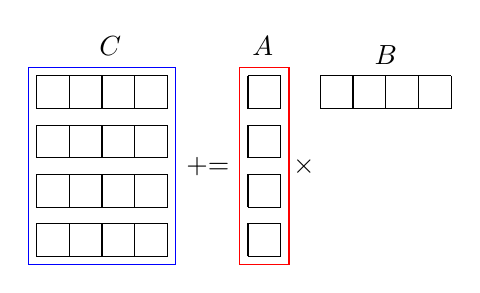
\begin{tikzpicture}[scale=5/12]
      \node[above=.75] at (2, 5.75) {$C$};
      \draw[shift={(-.25,0)}] (0,0) grid +(4,1);
      \draw[shift={(-.25,1.5)}] (0,0) grid +(4,1);
      \draw[shift={(-.25,3)}] (0,0) grid +(4,1);
      \draw[shift={(-.25,4.5)}] (0,0) grid +(4,1);
      \draw[shift={(-.5,-.25)},color=blue] (0, 0) -- +(4.5, 0) -- +(4.5, 6) -- +(0, 6) -- cycle;
      \node at (4.975,2.75) {$\mathrel{+}=$};
      \node[above=.75] at (6.65, 5.75) {$A$};
      \draw[shift={(6.2,0)}] (0,0) grid +(1,1);
      \draw[shift={(6.2,1.5)}] (0,0) grid +(1,1);
      \draw[shift={(6.2,3)}] (0,0) grid +(1,1);
      \draw[shift={(6.2,4.5)}] (0,0) grid +(1,1);
      \draw[shift={(5.95,-.25)},color=red] (0, 0) -- +(1.5, 0) -- +(1.5, 6) -- +(0, 6) -- cycle;
      \node at (7.9,2.75) {$\times$};
      \node[above=.75] at (10.4, 5.5) {$B$};
      \draw[shift={(8.4,4.5)}] (0,0) grid +(4,1);
    \end{tikzpicture}
    \caption{Extending block times panel.}
    \label{fig:extGebp}
  \end{subfigure}
  \hfill
  \begin{subfigure}{.5\linewidth}
    \centering
    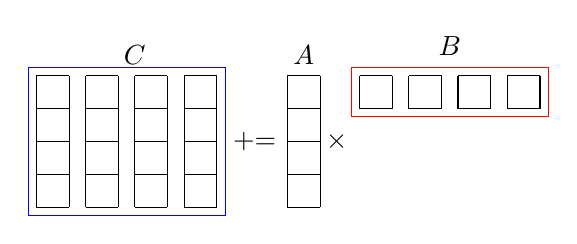
\begin{tikzpicture}[scale=5/12]
      \node[above=.75] at (2.75, 4) {$C$};
      \draw[shift={(-.25,0)}] (0,0) grid +(1,4);
      \draw[shift={(1.25,0)}] (0,0) grid +(1,4);
      \draw[shift={(2.74,0)}] (0,0) grid +(1,4);
      \draw[shift={(4.25,0)}] (0,0) grid +(1,4);
      \draw[shift={(-.5,-.25)},color=blue] (0, 0) -- +(6, 0) -- +(6, 4.5) -- +(0, 4.5) -- cycle;
      \node at (6.4,2) {$\mathrel{+}=$};
      \node[above=.75] at (7.9, 4) {$A$};
      \draw[shift={(7.4,0)}] (0,0) grid +(1,4);
      \node at (8.9,2) {$\times$};
      \node[above=.75] at (12.35, 4.25) {$B$};
      \draw[shift={(9.6,3)}] (0,0) grid +(1,1);
      \draw[shift={(11.1,3)}] (0,0) grid +(1,1);
      \draw[shift={(12.6,3)}] (0,0) grid +(1,1);
      \draw[shift={(14.1,3)}] (0,0) grid +(1,1);
      \draw[shift={(9.35,2.75)},color=red] (0, 0) -- +(6, 0) -- +(6, 1.5) -- +(0, 1.5) -- cycle;
    \end{tikzpicture}
    \caption{Extending panel times block.}
    \label{fig:extGepb}
  \end{subfigure}
  \hfill
  \caption[Extending inner kernels to outer product]{Extending Goto and van de Geijn's inner kernel techniques to outer product.}
  \label{fig:extGoto}
\end{figure}

\nelson{What is "this"?}
To improve this, the current operation must be reexamined.
In choosing this method, the implementer is performing a \matmul{1}{1}{n} or \matmul{n}{1}{1} matrix multiplication.
\nelson{What "it" refers to?}
While it is tempting to fall back to a traditional view of matrix multiplication and regard this as a simple inner product, a different point of view can be more beneficial.
\nelson{What does "this" refer to?}
Instead, we can choose to recognize this as a degenerate case of an outer product where one operand vector's length is one.
With this understanding, the direction for improvement becomes apparent.
The duplication issue can be resolved by replacing the duplicated values with unique values, extending the outer product's shortened dimension, bringing it closer to \rfig{outerProduct}.
Doing so stacks more of these operations, as shown in \rfig{extGoto}.
A red box represents one vector register, with each element therein being a distinct element from the matrix rather than a single \glslink{broadcast}{broadcasted} element.
Given a register that could contain the much larger output data in the blue boxes, the overhead of broadcasting can be completely removed.
\rcha{mma} shows how this is possible using \gls{power10}'s \gls{mma}.

\subsection{Implementation}
\bk{
  This section certainly repeats some previously discussed material.
  My hope is that in discussing it a second time, slightly more in depth, that it reinforces ideas instead of just being redundant.
  If you think it's redundant, please let me know.
}
As discussed previously, libraries often have kernels handwritten in assembly.
Kernel writers must implement all of these optimisations by hand.
In doing so, they must review \gls{cpu} properties as well as consider the design of their outer kernel to determine to what degree an optimisation will affect the hardware.
Historically, with great effort, this process has produced excellent results.

However, all of these optimisations and more are readily available in a compiler, often implemented generically and with great care regarding applicability and benefit analysis.
\bk{
  There's an example here that the default vectorisation lowering actually outputs a scalar version of matmul (simpler and easier to reason about/write) that's automatically vectorised by the compiler.
  However, I don't know that I can easily include it because it's based on intrinsics, lowerings, etc. that aren't explained until the method chapter.
}
Therefore, a kernel written within the compiler can be written at a higher and more generic level, as in an \gls{ir}, and achieve the same or better performance.
\bk{Section unfinished, got distracted by writing the previous section.}

\section{Usage cases}
\bk{
  Section to be removed per suggestion by Jo\~ao to link usage/motivation earlier.
  Leaving it as a reminder to do so.
}

\end{document}
